\documentclass[]{article}
\usepackage{lmodern}
\usepackage{amssymb,amsmath}
\usepackage{ifxetex,ifluatex}
\usepackage{fixltx2e} % provides \textsubscript
\ifnum 0\ifxetex 1\fi\ifluatex 1\fi=0 % if pdftex
  \usepackage[T1]{fontenc}
  \usepackage[utf8]{inputenc}
\else % if luatex or xelatex
  \ifxetex
    \usepackage{mathspec}
  \else
    \usepackage{fontspec}
  \fi
  \defaultfontfeatures{Ligatures=TeX,Scale=MatchLowercase}
\fi
% use upquote if available, for straight quotes in verbatim environments
\IfFileExists{upquote.sty}{\usepackage{upquote}}{}
% use microtype if available
\IfFileExists{microtype.sty}{%
\usepackage{microtype}
\UseMicrotypeSet[protrusion]{basicmath} % disable protrusion for tt fonts
}{}
\usepackage[margin=1in]{geometry}
\usepackage{hyperref}
\hypersetup{unicode=true,
            pdftitle={ANOVA desenvolvimento \textasciitilde{} area.de.conhecimento},
            pdfauthor={Geiser C. Challco geiser@usp.br},
            pdfborder={0 0 0},
            breaklinks=true}
\urlstyle{same}  % don't use monospace font for urls
\usepackage{color}
\usepackage{fancyvrb}
\newcommand{\VerbBar}{|}
\newcommand{\VERB}{\Verb[commandchars=\\\{\}]}
\DefineVerbatimEnvironment{Highlighting}{Verbatim}{commandchars=\\\{\}}
% Add ',fontsize=\small' for more characters per line
\usepackage{framed}
\definecolor{shadecolor}{RGB}{248,248,248}
\newenvironment{Shaded}{\begin{snugshade}}{\end{snugshade}}
\newcommand{\AlertTok}[1]{\textcolor[rgb]{0.94,0.16,0.16}{#1}}
\newcommand{\AnnotationTok}[1]{\textcolor[rgb]{0.56,0.35,0.01}{\textbf{\textit{#1}}}}
\newcommand{\AttributeTok}[1]{\textcolor[rgb]{0.77,0.63,0.00}{#1}}
\newcommand{\BaseNTok}[1]{\textcolor[rgb]{0.00,0.00,0.81}{#1}}
\newcommand{\BuiltInTok}[1]{#1}
\newcommand{\CharTok}[1]{\textcolor[rgb]{0.31,0.60,0.02}{#1}}
\newcommand{\CommentTok}[1]{\textcolor[rgb]{0.56,0.35,0.01}{\textit{#1}}}
\newcommand{\CommentVarTok}[1]{\textcolor[rgb]{0.56,0.35,0.01}{\textbf{\textit{#1}}}}
\newcommand{\ConstantTok}[1]{\textcolor[rgb]{0.00,0.00,0.00}{#1}}
\newcommand{\ControlFlowTok}[1]{\textcolor[rgb]{0.13,0.29,0.53}{\textbf{#1}}}
\newcommand{\DataTypeTok}[1]{\textcolor[rgb]{0.13,0.29,0.53}{#1}}
\newcommand{\DecValTok}[1]{\textcolor[rgb]{0.00,0.00,0.81}{#1}}
\newcommand{\DocumentationTok}[1]{\textcolor[rgb]{0.56,0.35,0.01}{\textbf{\textit{#1}}}}
\newcommand{\ErrorTok}[1]{\textcolor[rgb]{0.64,0.00,0.00}{\textbf{#1}}}
\newcommand{\ExtensionTok}[1]{#1}
\newcommand{\FloatTok}[1]{\textcolor[rgb]{0.00,0.00,0.81}{#1}}
\newcommand{\FunctionTok}[1]{\textcolor[rgb]{0.00,0.00,0.00}{#1}}
\newcommand{\ImportTok}[1]{#1}
\newcommand{\InformationTok}[1]{\textcolor[rgb]{0.56,0.35,0.01}{\textbf{\textit{#1}}}}
\newcommand{\KeywordTok}[1]{\textcolor[rgb]{0.13,0.29,0.53}{\textbf{#1}}}
\newcommand{\NormalTok}[1]{#1}
\newcommand{\OperatorTok}[1]{\textcolor[rgb]{0.81,0.36,0.00}{\textbf{#1}}}
\newcommand{\OtherTok}[1]{\textcolor[rgb]{0.56,0.35,0.01}{#1}}
\newcommand{\PreprocessorTok}[1]{\textcolor[rgb]{0.56,0.35,0.01}{\textit{#1}}}
\newcommand{\RegionMarkerTok}[1]{#1}
\newcommand{\SpecialCharTok}[1]{\textcolor[rgb]{0.00,0.00,0.00}{#1}}
\newcommand{\SpecialStringTok}[1]{\textcolor[rgb]{0.31,0.60,0.02}{#1}}
\newcommand{\StringTok}[1]{\textcolor[rgb]{0.31,0.60,0.02}{#1}}
\newcommand{\VariableTok}[1]{\textcolor[rgb]{0.00,0.00,0.00}{#1}}
\newcommand{\VerbatimStringTok}[1]{\textcolor[rgb]{0.31,0.60,0.02}{#1}}
\newcommand{\WarningTok}[1]{\textcolor[rgb]{0.56,0.35,0.01}{\textbf{\textit{#1}}}}
\usepackage{longtable,booktabs}
\usepackage{graphicx,grffile}
\makeatletter
\def\maxwidth{\ifdim\Gin@nat@width>\linewidth\linewidth\else\Gin@nat@width\fi}
\def\maxheight{\ifdim\Gin@nat@height>\textheight\textheight\else\Gin@nat@height\fi}
\makeatother
% Scale images if necessary, so that they will not overflow the page
% margins by default, and it is still possible to overwrite the defaults
% using explicit options in \includegraphics[width, height, ...]{}
\setkeys{Gin}{width=\maxwidth,height=\maxheight,keepaspectratio}
\IfFileExists{parskip.sty}{%
\usepackage{parskip}
}{% else
\setlength{\parindent}{0pt}
\setlength{\parskip}{6pt plus 2pt minus 1pt}
}
\setlength{\emergencystretch}{3em}  % prevent overfull lines
\providecommand{\tightlist}{%
  \setlength{\itemsep}{0pt}\setlength{\parskip}{0pt}}
\setcounter{secnumdepth}{0}
% Redefines (sub)paragraphs to behave more like sections
\ifx\paragraph\undefined\else
\let\oldparagraph\paragraph
\renewcommand{\paragraph}[1]{\oldparagraph{#1}\mbox{}}
\fi
\ifx\subparagraph\undefined\else
\let\oldsubparagraph\subparagraph
\renewcommand{\subparagraph}[1]{\oldsubparagraph{#1}\mbox{}}
\fi

%%% Use protect on footnotes to avoid problems with footnotes in titles
\let\rmarkdownfootnote\footnote%
\def\footnote{\protect\rmarkdownfootnote}

%%% Change title format to be more compact
\usepackage{titling}

% Create subtitle command for use in maketitle
\providecommand{\subtitle}[1]{
  \posttitle{
    \begin{center}\large#1\end{center}
    }
}

\setlength{\droptitle}{-2em}

  \title{ANOVA \texttt{desenvolvimento} \textasciitilde{}
\texttt{area.de.conhecimento}}
    \pretitle{\vspace{\droptitle}\centering\huge}
  \posttitle{\par}
    \author{Geiser C. Challco \href{mailto:geiser@usp.br}{\nolinkurl{geiser@usp.br}}}
    \preauthor{\centering\large\emph}
  \postauthor{\par}
    \date{}
    \predate{}\postdate{}
  

\begin{document}
\maketitle

\hypertarget{initial-data-and-preprocessing}{%
\subsection{Initial Data and
Preprocessing}\label{initial-data-and-preprocessing}}

R script: \url{factorialAnova.R} Inital data: \url{data.csv}

\hypertarget{summary-statistics-of-the-initial-data}{%
\subsubsection{Summary statistics of the initial
data}\label{summary-statistics-of-the-initial-data}}

\begin{Shaded}
\begin{Highlighting}[]
\KeywordTok{get_summary_stats}\NormalTok{(}\KeywordTok{group_by}\NormalTok{(dat, }\StringTok{`}\DataTypeTok{area.de.conhecimento}\StringTok{`}\NormalTok{), }\DataTypeTok{type =}\StringTok{"common"}\NormalTok{)}
\end{Highlighting}
\end{Shaded}

\begin{verbatim}
## # A tibble: 8 x 11
##   area.de.conheci~ variable     n   min   max median   iqr  mean    sd
##   <fct>            <chr>    <dbl> <dbl> <dbl>  <dbl> <dbl> <dbl> <dbl>
## 1 Ciências Agrári~ desenvo~    28  1.33  4.33   2.33  1     2.56 0.72 
## 2 Ciências Biológ~ desenvo~    22  1     4.33   2.33  1.33  2.32 0.832
## 3 Ciências da Saú~ desenvo~    65  1.33  5      3     1     2.83 0.802
## 4 Ciências Exatas~ desenvo~    48  1     4.33   2.67  1.42  2.57 0.891
## 5 Ciências Humanas desenvo~    45  1     4.33   2.67  1.33  2.66 0.812
## 6 Ciências Sociai~ desenvo~    53  1     4.33   2.67  1.33  2.65 0.867
## 7 Engenharias      desenvo~    31  1     4.67   2.67  1.33  2.67 0.873
## 8 Linguística/Let~ desenvo~    32  1     4.33   3     1.42  2.99 0.906
## # ... with 2 more variables: se <dbl>, ci <dbl>
\end{verbatim}

\hypertarget{check-assumptions}{%
\subsection{Check Assumptions}\label{check-assumptions}}

\hypertarget{identifying-outliers}{%
\subsubsection{Identifying outliers}\label{identifying-outliers}}

Outliers tend to increase type-I error probability, and they decrease
the calculated F statistic in ANOVA resulting in a lower chance of
reject the null hypothesis.

\begin{itemize}
\tightlist
\item
  Identified outliers using rstatix
\end{itemize}

\begin{Shaded}
\begin{Highlighting}[]
\KeywordTok{identify_outliers}\NormalTok{(}\KeywordTok{group_by}\NormalTok{(dat, }\StringTok{`}\DataTypeTok{area.de.conhecimento}\StringTok{`}\NormalTok{), }\StringTok{`}\DataTypeTok{desenvolvimento}\StringTok{`}\NormalTok{)}
\end{Highlighting}
\end{Shaded}

\begin{verbatim}
## # A tibble: 1 x 5
##   area.de.conhecimento ID     desenvolvimento is.outlier is.extreme
##   <fct>                <fct>            <dbl> <lgl>      <lgl>     
## 1 Ciências da Saúde    Obs322               5 TRUE       FALSE
\end{verbatim}

\begin{itemize}
\tightlist
\item
  Identified outliers through Boxplots
\end{itemize}

\begin{Shaded}
\begin{Highlighting}[]
\KeywordTok{Boxplot}\NormalTok{(}\StringTok{`}\DataTypeTok{desenvolvimento}\StringTok{`} \OperatorTok{~}\StringTok{ `}\DataTypeTok{area.de.conhecimento}\StringTok{`}\NormalTok{, }\DataTypeTok{data =}\NormalTok{ dat, }\DataTypeTok{id =} \KeywordTok{list}\NormalTok{(}\DataTypeTok{n =} \OtherTok{Inf}\NormalTok{))}
\end{Highlighting}
\end{Shaded}

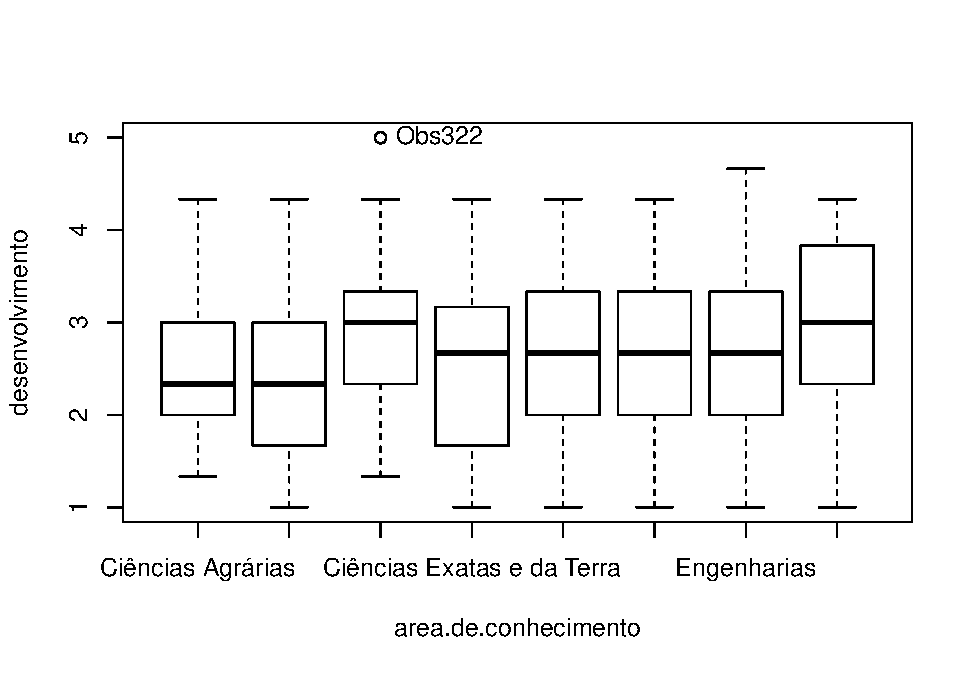
\includegraphics{factorialAnova_files/figure-latex/unnamed-chunk-3-1.pdf}

\begin{verbatim}
## [1] "Obs322"
\end{verbatim}

\hypertarget{removing-outliers-from-the-data}{%
\subsubsection{Removing outliers from the
data}\label{removing-outliers-from-the-data}}

\begin{Shaded}
\begin{Highlighting}[]
\NormalTok{outliers <-}\StringTok{ }\KeywordTok{c}\NormalTok{(}\StringTok{"Obs322"}\NormalTok{)}
\NormalTok{rdat <-}\StringTok{ }\NormalTok{dat[}\OperatorTok{!}\NormalTok{dat[[}\StringTok{"ID"}\NormalTok{]] }\OperatorTok\StringTok{ }\NormalTok{outliers,]   }\CommentTok{# table without outliers}
\end{Highlighting}
\end{Shaded}

\begin{longtable}[]{@{}lllr@{}}
\caption{Outliers table}\tabularnewline
\toprule
& ID & area.de.conhecimento & desenvolvimento\tabularnewline
\midrule
\endfirsthead
\toprule
& ID & area.de.conhecimento & desenvolvimento\tabularnewline
\midrule
\endhead
Obs322 & Obs322 & Ciências da Saúde & 5\tabularnewline
\bottomrule
\end{longtable}

\hypertarget{normality-assumption}{%
\subsubsection{Normality assumption}\label{normality-assumption}}

\textbf{Observation}:

As sample sizes increase, ANOVA remains a valid test even with the
violation of normality {[}\protect\hyperlink{references}{1},
\protect\hyperlink{references}{2}{]}. According to the central limit
theorem, the sampling distribution tends to be normal if the sample is
large enough (\texttt{n\ \textgreater{}\ 30}). Therefore, we performed
ANOVA with large samples as follows:

\begin{itemize}
\item
  In cases with the sample size greater than 30
  (\texttt{n\ \textgreater{}\ 30}), we adopted a significance level of
  \texttt{p\ \textless{}\ 0.01} instead a significance level of
  \texttt{p\ \textless{}\ 0.05}.
\item
  For samples with \texttt{n\ \textgreater{}\ 50} observation, we
  adopted D'Agostino-Pearson test that offers better accuracy for larger
  samples {[}\protect\hyperlink{references}{3}{]}.
\item
  For samples' size between \texttt{n\ \textgreater{}\ 100} and
  \texttt{n\ \textless{}=\ 200}, we ignored both tests (Shapiro and
  D'Agostino-Persons), and our decision of normality were based only in
  the interpretation of QQ-plots and histograms because these tests tend
  to be too sensitive with values greater than 200
  {[}\protect\hyperlink{references}{3}{]}.
\item
  For samples with \texttt{n\ \textgreater{}\ 200} observation, we
  ignore the normality assumption based on the central theorem limit,
  and taking only into account the homogeneity assumption.
\end{itemize}

\hypertarget{checking-normality-assumption-in-the-residual-model}{%
\paragraph{Checking normality assumption in the residual
model}\label{checking-normality-assumption-in-the-residual-model}}

\begin{Shaded}
\begin{Highlighting}[]
\NormalTok{mdl <-}\StringTok{ }\KeywordTok{lm}\NormalTok{(}\StringTok{`}\DataTypeTok{desenvolvimento}\StringTok{`} \OperatorTok{~}\StringTok{ `}\DataTypeTok{area.de.conhecimento}\StringTok{`}\NormalTok{, }\DataTypeTok{data =}\NormalTok{ rdat)}
\KeywordTok{normality_test}\NormalTok{(}\KeywordTok{residuals}\NormalTok{(mdl))}
\end{Highlighting}
\end{Shaded}

\begin{verbatim}
##     n statistic     method           p p.signif normality
## 1 323  10.27096 D'Agostino 0.005884222        *         -
\end{verbatim}

The QQ plot used to evaluate normality assumption

\begin{Shaded}
\begin{Highlighting}[]
\KeywordTok{qqPlot}\NormalTok{(}\KeywordTok{residuals}\NormalTok{(mdl))}
\end{Highlighting}
\end{Shaded}

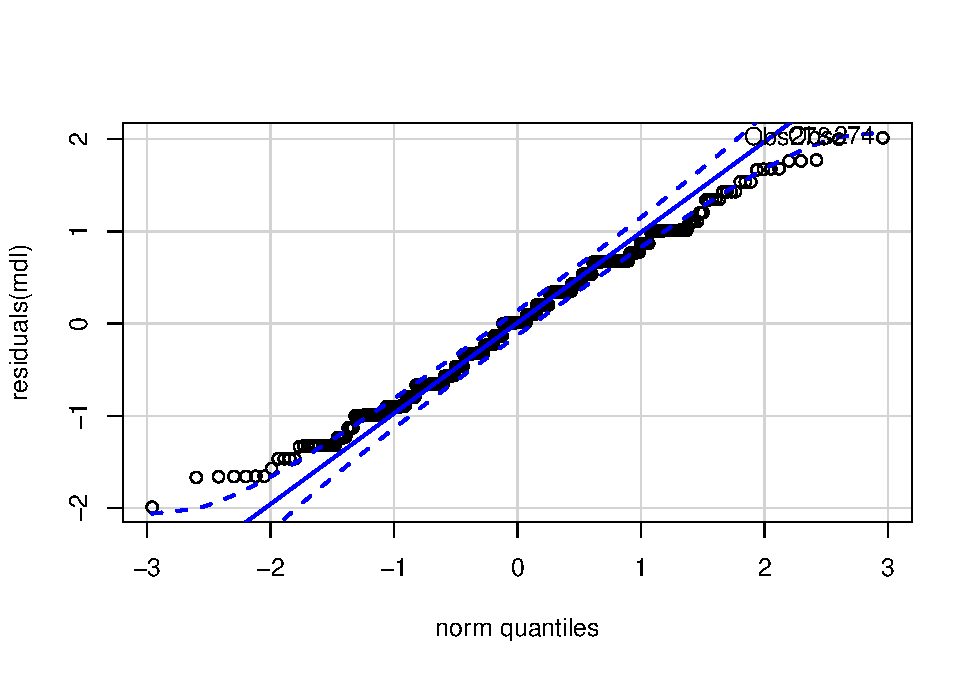
\includegraphics{factorialAnova_files/figure-latex/unnamed-chunk-7-1.pdf}

\begin{verbatim}
## Obs274 Obs278 
##    268    272
\end{verbatim}

\hypertarget{checking-normality-assumption-for-each-group}{%
\paragraph{Checking normality assumption for each
group}\label{checking-normality-assumption-for-each-group}}

\begin{Shaded}
\begin{Highlighting}[]
\KeywordTok{normality_test_at}\NormalTok{(}\KeywordTok{group_by}\NormalTok{(rdat, }\StringTok{`}\DataTypeTok{area.de.conhecimento}\StringTok{`}\NormalTok{), }\StringTok{"desenvolvimento"}\NormalTok{)}
\end{Highlighting}
\end{Shaded}

\begin{verbatim}
##                       variable       area.de.conhecimento  n statistic
## 1              desenvolvimento          Ciências Agrárias 28 0.9597002
## 2              desenvolvimento        Ciências Biológicas 22 0.9298277
## Omnibus  Test  desenvolvimento          Ciências da Saúde 64 0.6215602
## 11             desenvolvimento Ciências Exatas e da Terra 48 0.9474154
## 12             desenvolvimento           Ciências Humanas 45 0.9642608
## Omnibus  Test1 desenvolvimento Ciências Sociais Aplicadas 53 1.7440391
## 13             desenvolvimento                Engenharias 31 0.9685706
## 14             desenvolvimento Linguística/Letras e Artes 32 0.9358006
##                      method          p p.signif normality
## 1              Shapiro-Wilk 0.34300413       ns       YES
## 2              Shapiro-Wilk 0.12168686       ns       YES
## Omnibus  Test    D'Agostino 0.73287501       ns       YES
## 11             Shapiro-Wilk 0.03157974       ns       YES
## 12             Shapiro-Wilk 0.17733217       ns       YES
## Omnibus  Test1   D'Agostino 0.41810630       ns       YES
## 13             Shapiro-Wilk 0.48060883       ns       YES
## 14             Shapiro-Wilk 0.05694906       ns       YES
\end{verbatim}

\begin{itemize}
\tightlist
\item
  QQ plot in the \textbf{area.de.conhecimento}: ``Ciências Agrárias''
\end{itemize}

\begin{Shaded}
\begin{Highlighting}[]
\KeywordTok{qqPlot}\NormalTok{( }\OperatorTok{~}\StringTok{ `}\DataTypeTok{desenvolvimento}\StringTok{`}\NormalTok{, }\DataTypeTok{data =}\NormalTok{ rdat[}\KeywordTok{which}\NormalTok{(rdat[}\StringTok{"area.de.conhecimento"}\NormalTok{] }\OperatorTok{==}\StringTok{ "Ciências Agrárias"}\NormalTok{),])}
\end{Highlighting}
\end{Shaded}

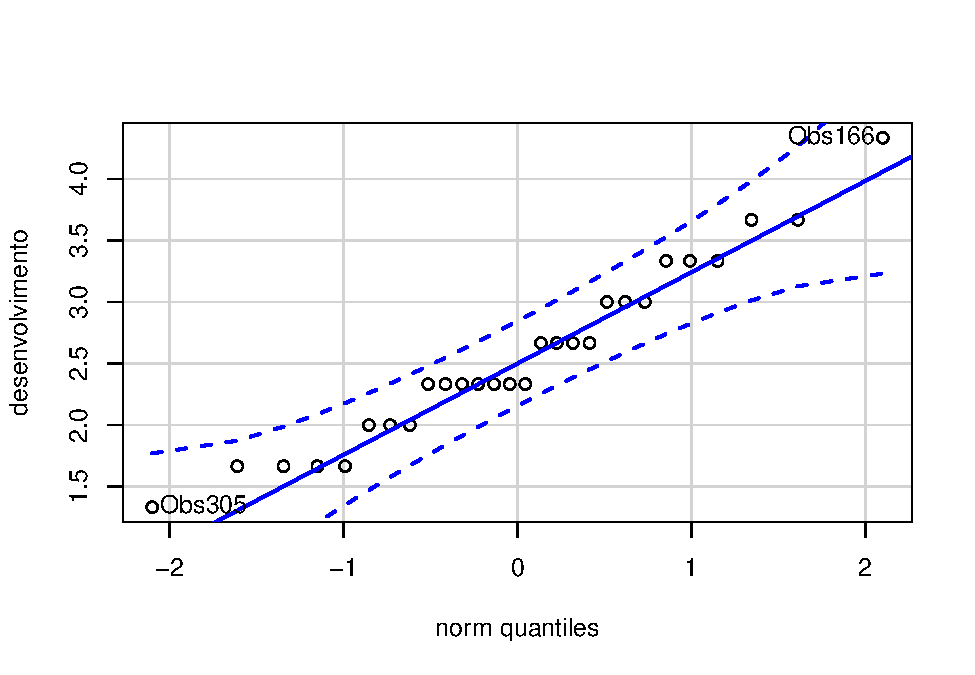
\includegraphics{factorialAnova_files/figure-latex/unnamed-chunk-9-1.pdf}

\begin{verbatim}
## Obs166 Obs305 
##     15     27
\end{verbatim}

\begin{itemize}
\tightlist
\item
  QQ plot in the \textbf{area.de.conhecimento}: ``Ciências Biológicas''
\end{itemize}

\begin{Shaded}
\begin{Highlighting}[]
\KeywordTok{qqPlot}\NormalTok{( }\OperatorTok{~}\StringTok{ `}\DataTypeTok{desenvolvimento}\StringTok{`}\NormalTok{, }\DataTypeTok{data =}\NormalTok{ rdat[}\KeywordTok{which}\NormalTok{(rdat[}\StringTok{"area.de.conhecimento"}\NormalTok{] }\OperatorTok{==}\StringTok{ "Ciências Biológicas"),])}
\end{Highlighting}
\end{Shaded}

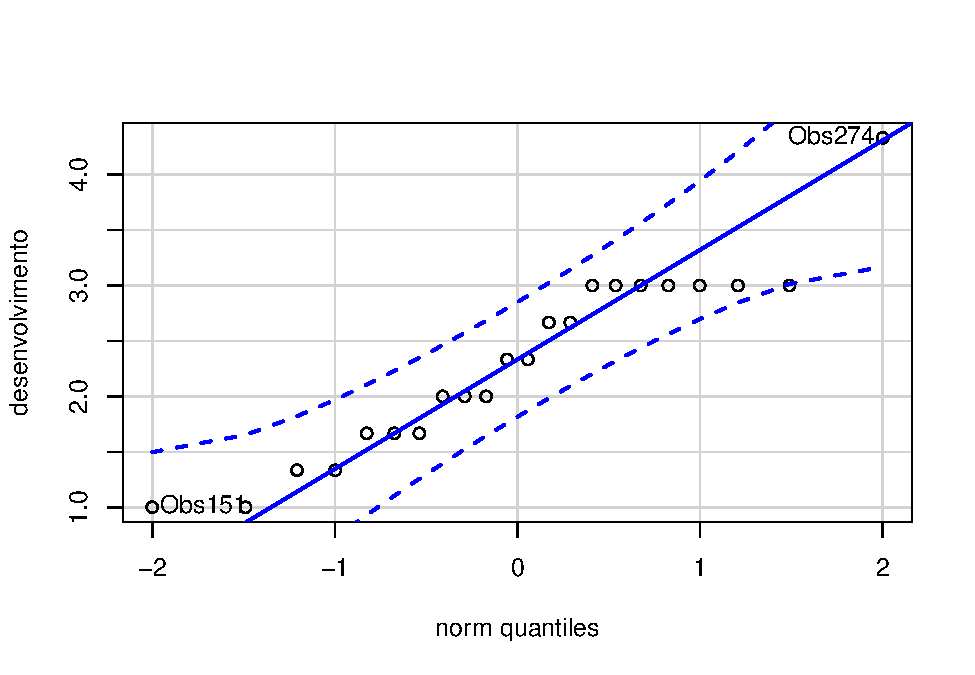
\includegraphics{factorialAnova_files/figure-latex/unnamed-chunk-10-1.pdf}

\begin{verbatim}
## Obs274 Obs151 
##     20      9
\end{verbatim}

\begin{itemize}
\tightlist
\item
  QQ plot in the \textbf{area.de.conhecimento}: ``Ciências da Saúde''
\end{itemize}

\begin{Shaded}
\begin{Highlighting}[]
\KeywordTok{qqPlot}\NormalTok{( }\OperatorTok{~}\StringTok{ `}\DataTypeTok{desenvolvimento}\StringTok{`}\NormalTok{, }\DataTypeTok{data =}\NormalTok{ rdat[}\KeywordTok{which}\NormalTok{(rdat[}\StringTok{"area.de.conhecimento"}\NormalTok{] }\OperatorTok{==}\StringTok{ "Ciências da Saúde"),])}
\end{Highlighting}
\end{Shaded}

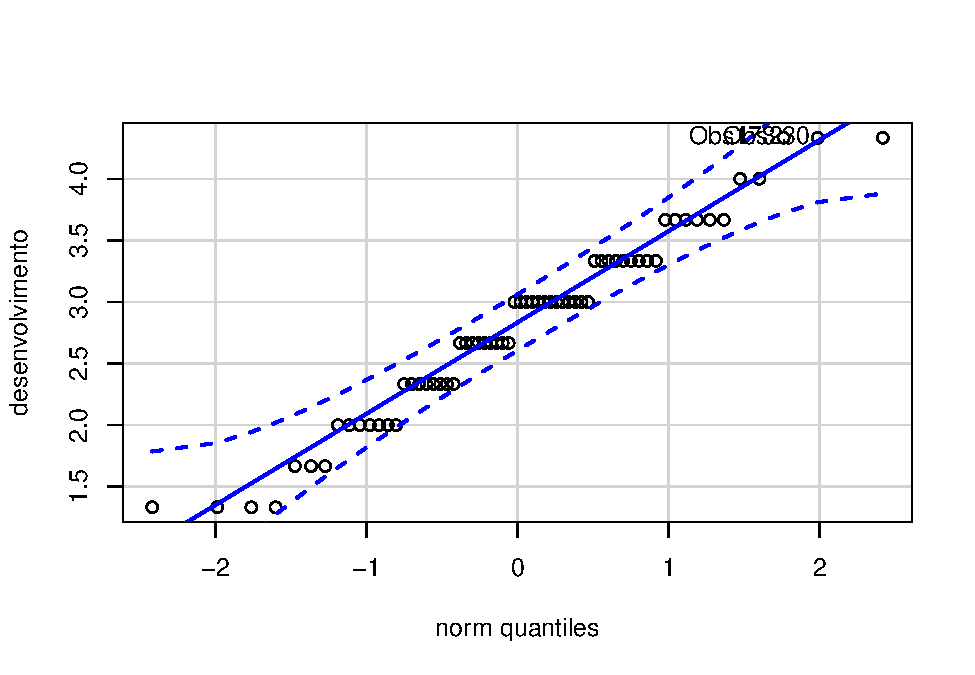
\includegraphics{factorialAnova_files/figure-latex/unnamed-chunk-11-1.pdf}

\begin{verbatim}
## Obs173 Obs230 
##     27     37
\end{verbatim}

\begin{itemize}
\tightlist
\item
  QQ plot in the \textbf{area.de.conhecimento}: ``Ciências Exatas e da
  Terra''
\end{itemize}

\begin{Shaded}
\begin{Highlighting}[]
\KeywordTok{qqPlot}\NormalTok{( }\OperatorTok{~}\StringTok{ `}\DataTypeTok{desenvolvimento}\StringTok{`}\NormalTok{, }\DataTypeTok{data =}\NormalTok{ rdat[}\KeywordTok{which}\NormalTok{(rdat[}\StringTok{"area.de.conhecimento"}\NormalTok{] }\OperatorTok{==}\StringTok{ "Ciências Exatas e da Terra"}\NormalTok{),])}
\end{Highlighting}
\end{Shaded}

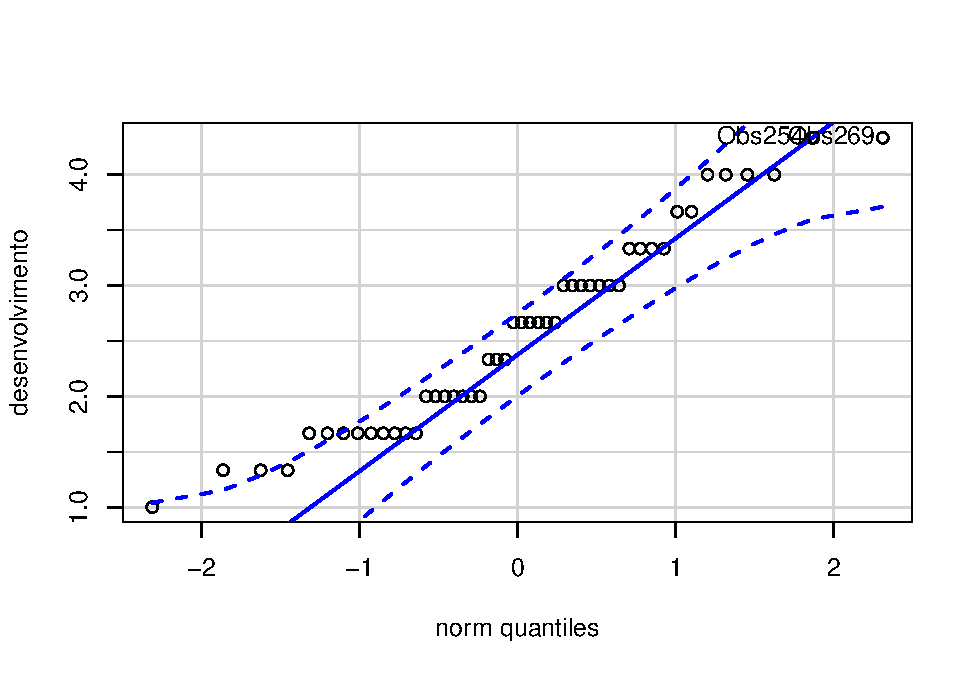
\includegraphics{factorialAnova_files/figure-latex/unnamed-chunk-12-1.pdf}

\begin{verbatim}
## Obs254 Obs269 
##     35     38
\end{verbatim}

\begin{itemize}
\tightlist
\item
  QQ plot in the \textbf{area.de.conhecimento}: ``Ciências Humanas''
\end{itemize}

\begin{Shaded}
\begin{Highlighting}[]
\KeywordTok{qqPlot}\NormalTok{( }\OperatorTok{~}\StringTok{ `}\DataTypeTok{desenvolvimento}\StringTok{`}\NormalTok{, }\DataTypeTok{data =}\NormalTok{ rdat[}\KeywordTok{which}\NormalTok{(rdat[}\StringTok{"area.de.conhecimento"}\NormalTok{] }\OperatorTok{==}\StringTok{ "Ciências Humanas"}\NormalTok{),])}
\end{Highlighting}
\end{Shaded}

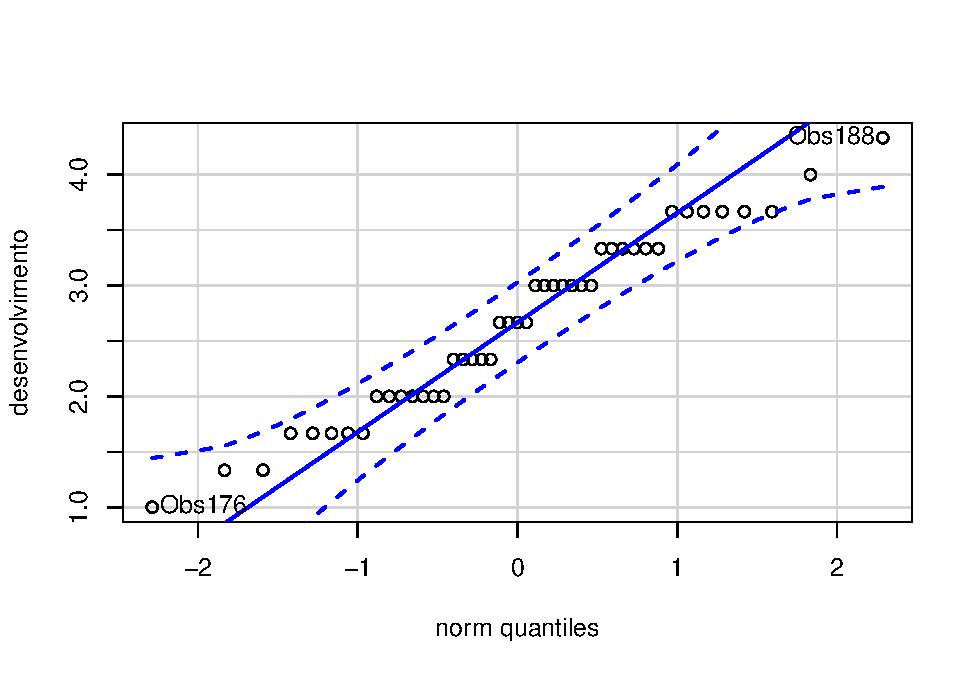
\includegraphics{factorialAnova_files/figure-latex/unnamed-chunk-13-1.pdf}

\begin{verbatim}
## Obs188 Obs176 
##     33     30
\end{verbatim}

\begin{itemize}
\tightlist
\item
  QQ plot in the \textbf{area.de.conhecimento}: ``Ciências Sociais
  Aplicadas''
\end{itemize}

\begin{Shaded}
\begin{Highlighting}[]
\KeywordTok{qqPlot}\NormalTok{( }\OperatorTok{~}\StringTok{ `}\DataTypeTok{desenvolvimento}\StringTok{`}\NormalTok{, }\DataTypeTok{data =}\NormalTok{ rdat[}\KeywordTok{which}\NormalTok{(rdat[}\StringTok{"area.de.conhecimento"}\NormalTok{] }\OperatorTok{==}\StringTok{ "Ciências Sociais Aplicadas"}\NormalTok{),])}
\end{Highlighting}
\end{Shaded}

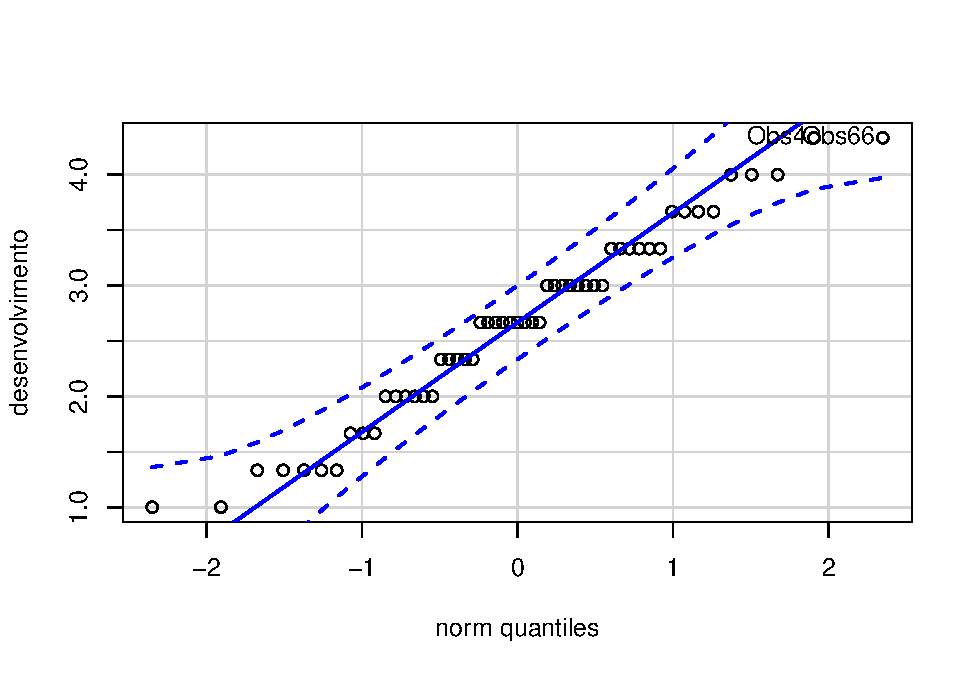
\includegraphics{factorialAnova_files/figure-latex/unnamed-chunk-14-1.pdf}

\begin{verbatim}
##  Obs4 Obs66 
##     2    22
\end{verbatim}

\begin{itemize}
\tightlist
\item
  QQ plot in the \textbf{area.de.conhecimento}: ``Engenharias''
\end{itemize}

\begin{Shaded}
\begin{Highlighting}[]
\KeywordTok{qqPlot}\NormalTok{( }\OperatorTok{~}\StringTok{ `}\DataTypeTok{desenvolvimento}\StringTok{`}\NormalTok{, }\DataTypeTok{data =}\NormalTok{ rdat[}\KeywordTok{which}\NormalTok{(rdat[}\StringTok{"area.de.conhecimento"}\NormalTok{] }\OperatorTok{==}\StringTok{ "Engenharias"}\NormalTok{),])}
\end{Highlighting}
\end{Shaded}

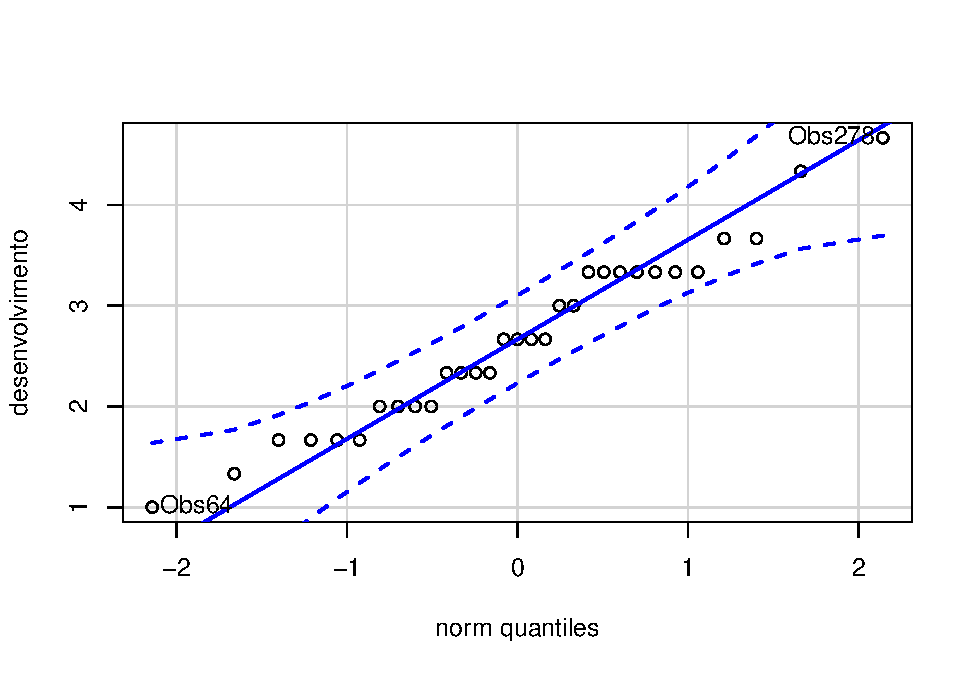
\includegraphics{factorialAnova_files/figure-latex/unnamed-chunk-15-1.pdf}

\begin{verbatim}
## Obs278  Obs64 
##     24      7
\end{verbatim}

\begin{itemize}
\tightlist
\item
  QQ plot in the \textbf{area.de.conhecimento}: ``Linguística/Letras e
  Artes''
\end{itemize}

\begin{Shaded}
\begin{Highlighting}[]
\KeywordTok{qqPlot}\NormalTok{( }\OperatorTok{~}\StringTok{ `}\DataTypeTok{desenvolvimento}\StringTok{`}\NormalTok{, }\DataTypeTok{data =}\NormalTok{ rdat[}\KeywordTok{which}\NormalTok{(rdat[}\StringTok{"area.de.conhecimento"}\NormalTok{] }\OperatorTok{==}\StringTok{ "Linguística/Letras e Artes"}\NormalTok{),])}
\end{Highlighting}
\end{Shaded}

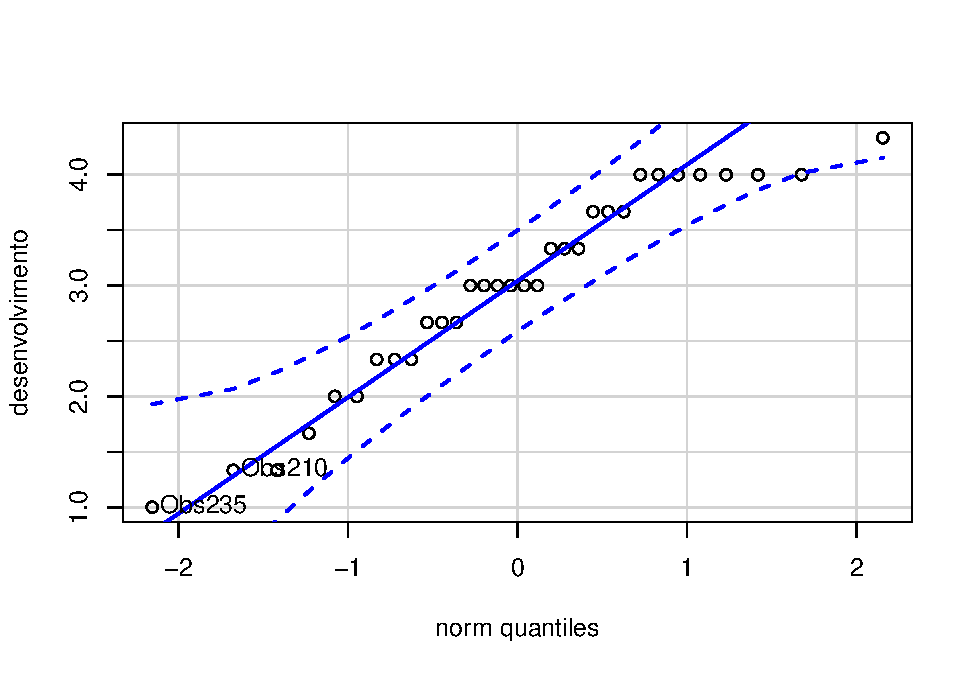
\includegraphics{factorialAnova_files/figure-latex/unnamed-chunk-16-1.pdf}

\begin{verbatim}
## Obs235 Obs210 
##     24     13
\end{verbatim}

\hypertarget{removing-data-that-affect-normality}{%
\paragraph{Removing data that affect
normality}\label{removing-data-that-affect-normality}}

\begin{Shaded}
\begin{Highlighting}[]
\NormalTok{non.normal <-}\StringTok{ }\KeywordTok{c}\NormalTok{(}\StringTok{""}\NormalTok{)}
\NormalTok{sdat <-}\StringTok{ }\NormalTok{rdat[}\OperatorTok{!}\NormalTok{rdat[[}\StringTok{"ID"}\NormalTok{]] }\OperatorTok\StringTok{ }\NormalTok{non.normal,]   }\CommentTok{# table without non-normal and outliers}
\end{Highlighting}
\end{Shaded}

\begin{longtable}[]{@{}llr@{}}
\caption{Non-normal data table}\tabularnewline
\toprule
ID & area.de.conhecimento & desenvolvimento\tabularnewline
\midrule
\endfirsthead
\toprule
ID & area.de.conhecimento & desenvolvimento\tabularnewline
\midrule
\endhead
\bottomrule
\end{longtable}

\hypertarget{performing-normality-test-without-data-that-affect-normality}{%
\paragraph{Performing normality test without data that affect
normality}\label{performing-normality-test-without-data-that-affect-normality}}

\begin{Shaded}
\begin{Highlighting}[]
\NormalTok{mdl <-}\StringTok{ }\KeywordTok{lm}\NormalTok{(}\StringTok{`}\DataTypeTok{desenvolvimento}\StringTok{`} \OperatorTok{~}\StringTok{ `}\DataTypeTok{area.de.conhecimento}\StringTok{`}\NormalTok{, }\DataTypeTok{data =}\NormalTok{ sdat)}
\KeywordTok{normality_test}\NormalTok{(}\KeywordTok{residuals}\NormalTok{(mdl))}
\end{Highlighting}
\end{Shaded}

\begin{longtable}[]{@{}rrllll@{}}
\toprule
n & statistic & method & p & p.signif & normality\tabularnewline
\midrule
\endhead
323 & 10.271 & D'Agostino & 0.0059 & * & -\tabularnewline
\bottomrule
\end{longtable}

\begin{Shaded}
\begin{Highlighting}[]
\KeywordTok{normality_test_at}\NormalTok{(}\KeywordTok{group_by}\NormalTok{(sdat, }\StringTok{`}\DataTypeTok{area.de.conhecimento}\StringTok{`}\NormalTok{), }\StringTok{"desenvolvimento"}\NormalTok{)}
\end{Highlighting}
\end{Shaded}

\begin{longtable}[]{@{}llrrllll@{}}
\toprule
variable & area.de.conhecimento & n & statistic & method & p & p.signif
& normality\tabularnewline
\midrule
\endhead
desenvolvimento & Ciências Agrárias & 28 & 0.9597 & Shapiro-Wilk & 0.343
& ns & YES\tabularnewline
desenvolvimento & Ciências Biológicas & 22 & 0.9298 & Shapiro-Wilk &
0.1217 & ns & YES\tabularnewline
desenvolvimento & Ciências da Saúde & 64 & 0.6216 & D'Agostino & 0.7329
& ns & YES\tabularnewline
desenvolvimento & Ciências Exatas e da Terra & 48 & 0.9474 &
Shapiro-Wilk & 0.0316 & * & YES\tabularnewline
desenvolvimento & Ciências Humanas & 45 & 0.9643 & Shapiro-Wilk & 0.1773
& ns & YES\tabularnewline
desenvolvimento & Ciências Sociais Aplicadas & 53 & 1.7440 & D'Agostino
& 0.4181 & ns & YES\tabularnewline
desenvolvimento & Engenharias & 31 & 0.9686 & Shapiro-Wilk & 0.4806 & ns
& YES\tabularnewline
desenvolvimento & Linguística/Letras e Artes & 32 & 0.9358 &
Shapiro-Wilk & 0.0569 & ns & YES\tabularnewline
\bottomrule
\end{longtable}

QQ plot in the residual model without data that affect normality

\begin{Shaded}
\begin{Highlighting}[]
\KeywordTok{qqPlot}\NormalTok{(}\KeywordTok{residuals}\NormalTok{(mdl))}
\end{Highlighting}
\end{Shaded}

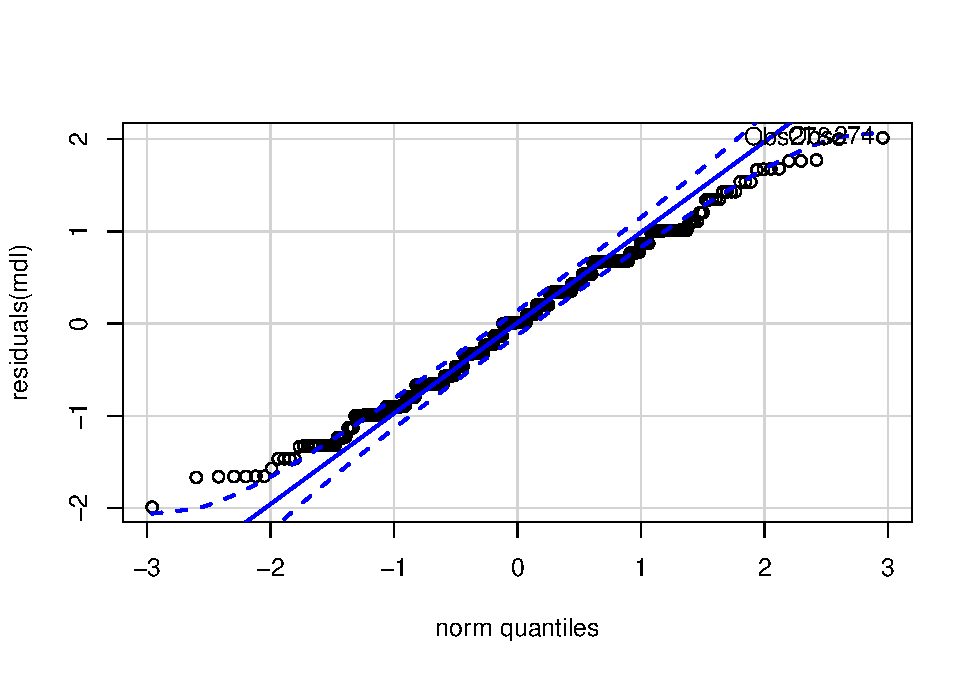
\includegraphics{factorialAnova_files/figure-latex/unnamed-chunk-21-1.pdf}

\begin{verbatim}
## Obs274 Obs278 
##    268    272
\end{verbatim}

\begin{itemize}
\tightlist
\item
  QQ plot in the \textbf{area.de.conhecimento}: ``Ciências Agrárias''
\end{itemize}

\begin{Shaded}
\begin{Highlighting}[]
\KeywordTok{qqPlot}\NormalTok{( }\OperatorTok{~}\StringTok{ `}\DataTypeTok{desenvolvimento}\StringTok{`}\NormalTok{, }\DataTypeTok{data =}\NormalTok{ sdat[}\KeywordTok{which}\NormalTok{(sdat[}\StringTok{"area.de.conhecimento"}\NormalTok{] }\OperatorTok{==}\StringTok{ "Ciências Agrárias"}\NormalTok{),])}
\end{Highlighting}
\end{Shaded}

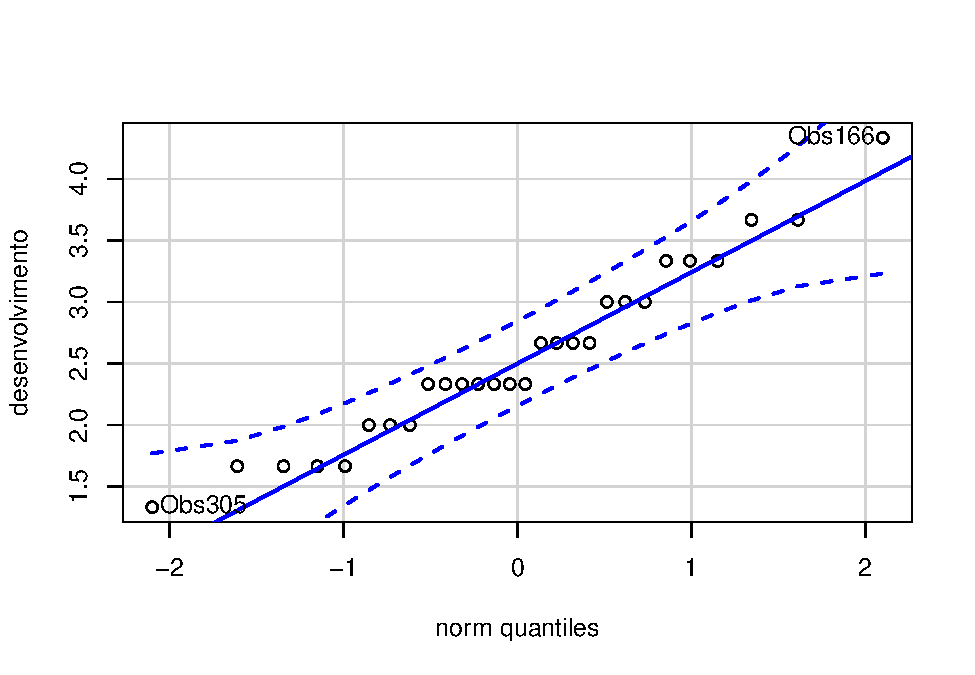
\includegraphics{factorialAnova_files/figure-latex/unnamed-chunk-22-1.pdf}

\begin{verbatim}
## Obs166 Obs305 
##     15     27
\end{verbatim}

\begin{itemize}
\tightlist
\item
  QQ plot in the \textbf{area.de.conhecimento}: ``Ciências Biológicas''
\end{itemize}

\begin{Shaded}
\begin{Highlighting}[]
\KeywordTok{qqPlot}\NormalTok{( }\OperatorTok{~}\StringTok{ `}\DataTypeTok{desenvolvimento}\StringTok{`}\NormalTok{, }\DataTypeTok{data =}\NormalTok{ sdat[}\KeywordTok{which}\NormalTok{(sdat[}\StringTok{"area.de.conhecimento"}\NormalTok{] }\OperatorTok{==}\StringTok{ "Ciências Biológicas"),])}
\end{Highlighting}
\end{Shaded}

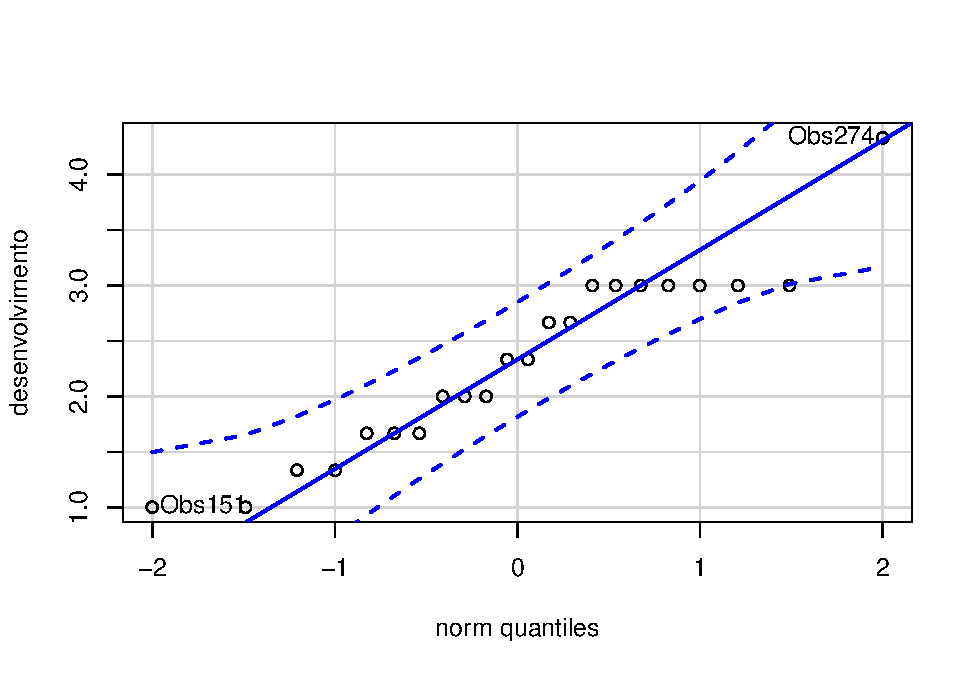
\includegraphics{factorialAnova_files/figure-latex/unnamed-chunk-23-1.pdf}

\begin{verbatim}
## Obs274 Obs151 
##     20      9
\end{verbatim}

\begin{itemize}
\tightlist
\item
  QQ plot in the \textbf{area.de.conhecimento}: ``Ciências da Saúde''
\end{itemize}

\begin{Shaded}
\begin{Highlighting}[]
\KeywordTok{qqPlot}\NormalTok{( }\OperatorTok{~}\StringTok{ `}\DataTypeTok{desenvolvimento}\StringTok{`}\NormalTok{, }\DataTypeTok{data =}\NormalTok{ sdat[}\KeywordTok{which}\NormalTok{(sdat[}\StringTok{"area.de.conhecimento"}\NormalTok{] }\OperatorTok{==}\StringTok{ "Ciências da Saúde"),])}
\end{Highlighting}
\end{Shaded}

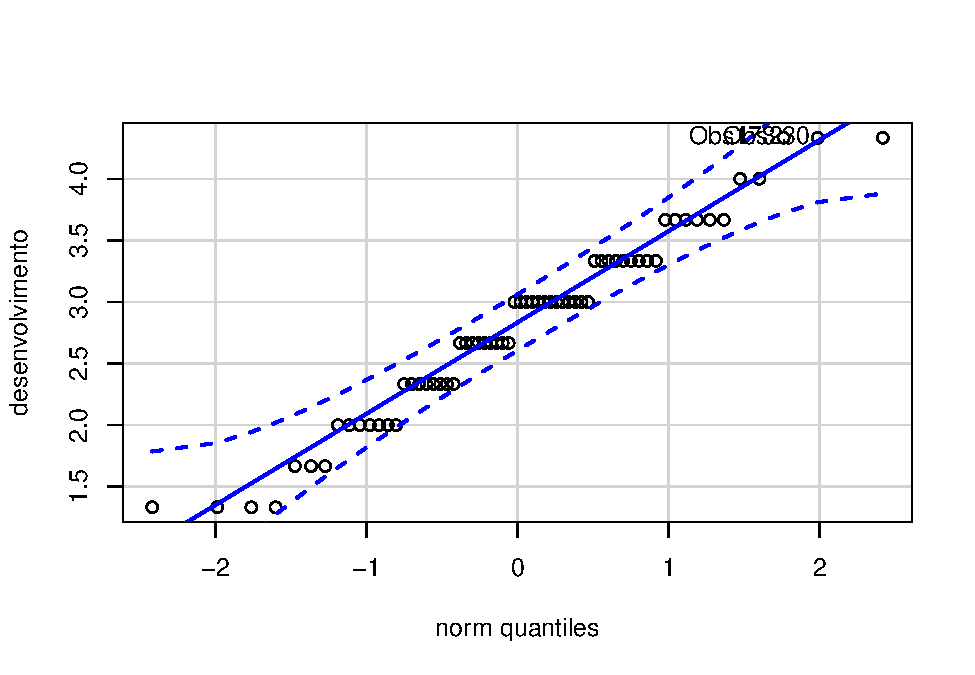
\includegraphics{factorialAnova_files/figure-latex/unnamed-chunk-24-1.pdf}

\begin{verbatim}
## Obs173 Obs230 
##     27     37
\end{verbatim}

\begin{itemize}
\tightlist
\item
  QQ plot in the \textbf{area.de.conhecimento}: ``Ciências Exatas e da
  Terra''
\end{itemize}

\begin{Shaded}
\begin{Highlighting}[]
\KeywordTok{qqPlot}\NormalTok{( }\OperatorTok{~}\StringTok{ `}\DataTypeTok{desenvolvimento}\StringTok{`}\NormalTok{, }\DataTypeTok{data =}\NormalTok{ sdat[}\KeywordTok{which}\NormalTok{(sdat[}\StringTok{"area.de.conhecimento"}\NormalTok{] }\OperatorTok{==}\StringTok{ "Ciências Exatas e da Terra"}\NormalTok{),])}
\end{Highlighting}
\end{Shaded}

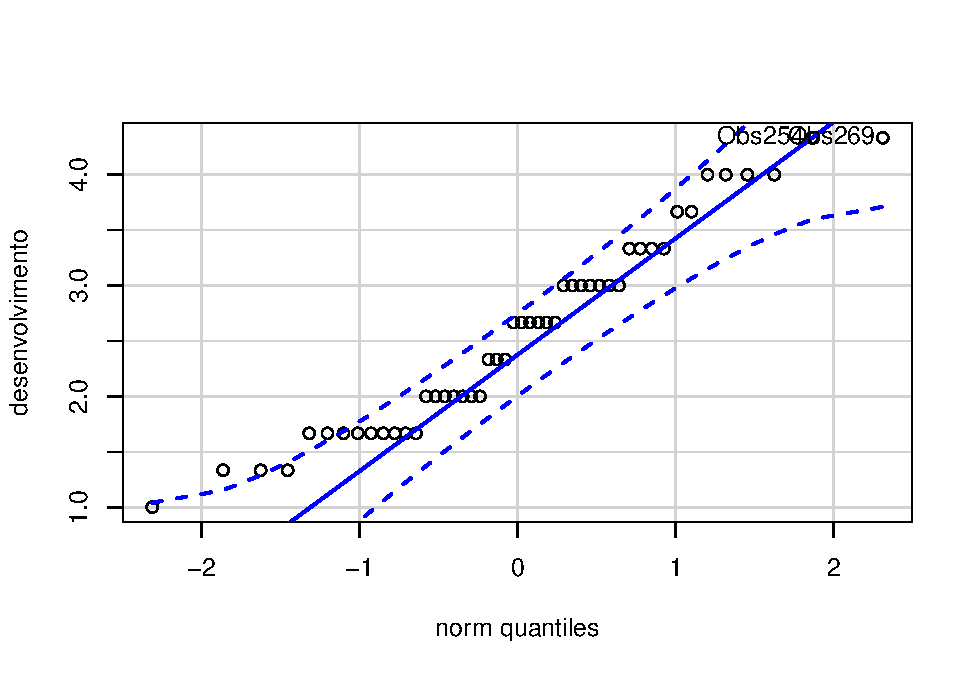
\includegraphics{factorialAnova_files/figure-latex/unnamed-chunk-25-1.pdf}

\begin{verbatim}
## Obs254 Obs269 
##     35     38
\end{verbatim}

\begin{itemize}
\tightlist
\item
  QQ plot in the \textbf{area.de.conhecimento}: ``Ciências Humanas''
\end{itemize}

\begin{Shaded}
\begin{Highlighting}[]
\KeywordTok{qqPlot}\NormalTok{( }\OperatorTok{~}\StringTok{ `}\DataTypeTok{desenvolvimento}\StringTok{`}\NormalTok{, }\DataTypeTok{data =}\NormalTok{ sdat[}\KeywordTok{which}\NormalTok{(sdat[}\StringTok{"area.de.conhecimento"}\NormalTok{] }\OperatorTok{==}\StringTok{ "Ciências Humanas"}\NormalTok{),])}
\end{Highlighting}
\end{Shaded}

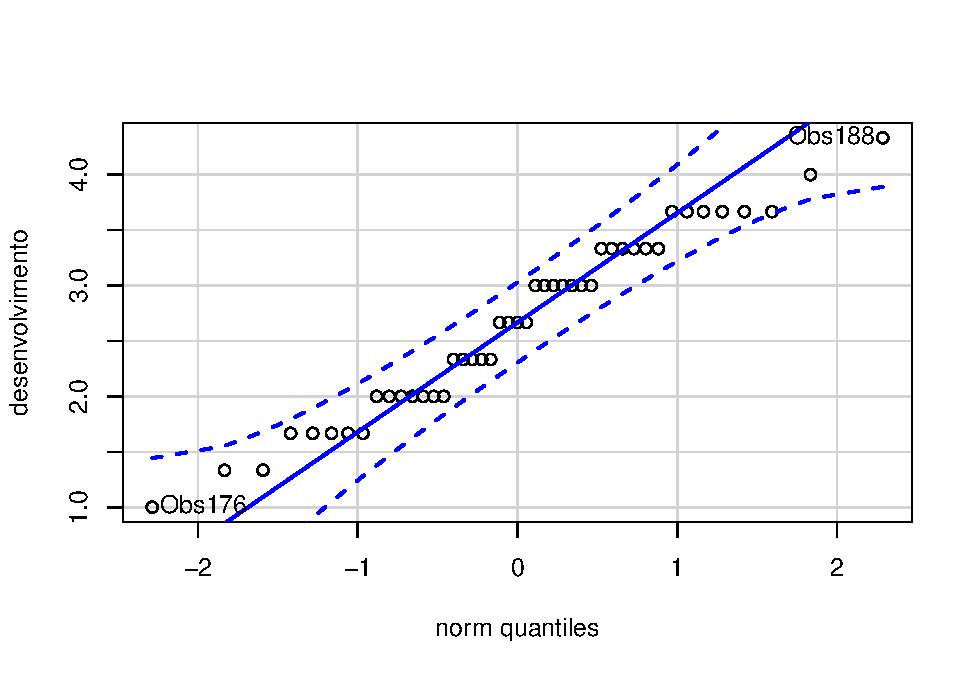
\includegraphics{factorialAnova_files/figure-latex/unnamed-chunk-26-1.pdf}

\begin{verbatim}
## Obs188 Obs176 
##     33     30
\end{verbatim}

\begin{itemize}
\tightlist
\item
  QQ plot in the \textbf{area.de.conhecimento}: ``Ciências Sociais
  Aplicadas''
\end{itemize}

\begin{Shaded}
\begin{Highlighting}[]
\KeywordTok{qqPlot}\NormalTok{( }\OperatorTok{~}\StringTok{ `}\DataTypeTok{desenvolvimento}\StringTok{`}\NormalTok{, }\DataTypeTok{data =}\NormalTok{ sdat[}\KeywordTok{which}\NormalTok{(sdat[}\StringTok{"area.de.conhecimento"}\NormalTok{] }\OperatorTok{==}\StringTok{ "Ciências Sociais Aplicadas"}\NormalTok{),])}
\end{Highlighting}
\end{Shaded}

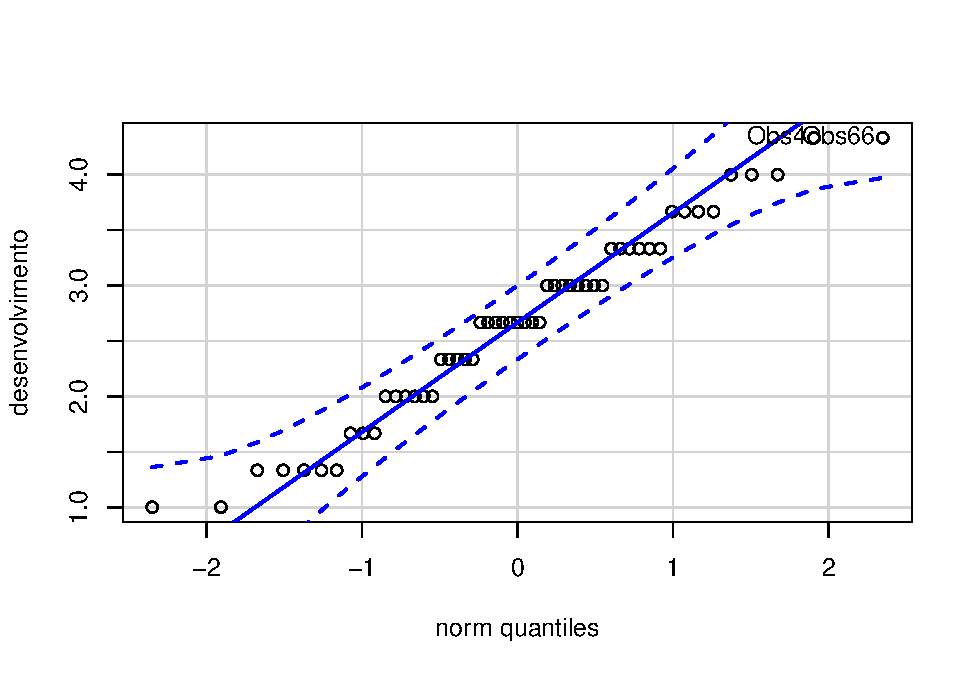
\includegraphics{factorialAnova_files/figure-latex/unnamed-chunk-27-1.pdf}

\begin{verbatim}
##  Obs4 Obs66 
##     2    22
\end{verbatim}

\begin{itemize}
\tightlist
\item
  QQ plot in the \textbf{area.de.conhecimento}: ``Engenharias''
\end{itemize}

\begin{Shaded}
\begin{Highlighting}[]
\KeywordTok{qqPlot}\NormalTok{( }\OperatorTok{~}\StringTok{ `}\DataTypeTok{desenvolvimento}\StringTok{`}\NormalTok{, }\DataTypeTok{data =}\NormalTok{ sdat[}\KeywordTok{which}\NormalTok{(sdat[}\StringTok{"area.de.conhecimento"}\NormalTok{] }\OperatorTok{==}\StringTok{ "Engenharias"}\NormalTok{),])}
\end{Highlighting}
\end{Shaded}

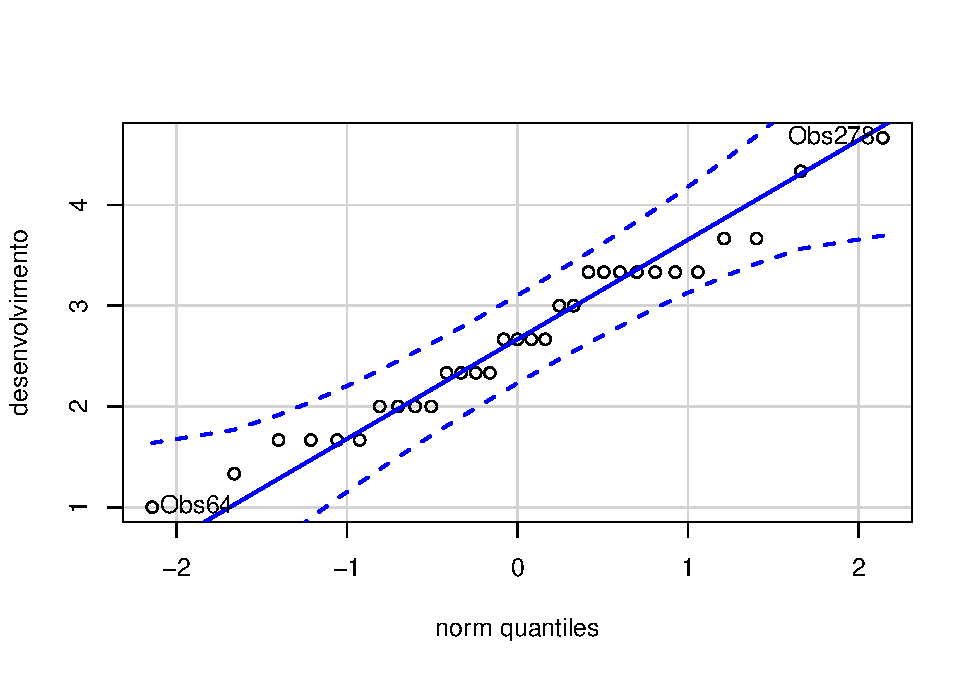
\includegraphics{factorialAnova_files/figure-latex/unnamed-chunk-28-1.pdf}

\begin{verbatim}
## Obs278  Obs64 
##     24      7
\end{verbatim}

\begin{itemize}
\tightlist
\item
  QQ plot in the \textbf{area.de.conhecimento}: ``Linguística/Letras e
  Artes''
\end{itemize}

\begin{Shaded}
\begin{Highlighting}[]
\KeywordTok{qqPlot}\NormalTok{( }\OperatorTok{~}\StringTok{ `}\DataTypeTok{desenvolvimento}\StringTok{`}\NormalTok{, }\DataTypeTok{data =}\NormalTok{ sdat[}\KeywordTok{which}\NormalTok{(sdat[}\StringTok{"area.de.conhecimento"}\NormalTok{] }\OperatorTok{==}\StringTok{ "Linguística/Letras e Artes"}\NormalTok{),])}
\end{Highlighting}
\end{Shaded}

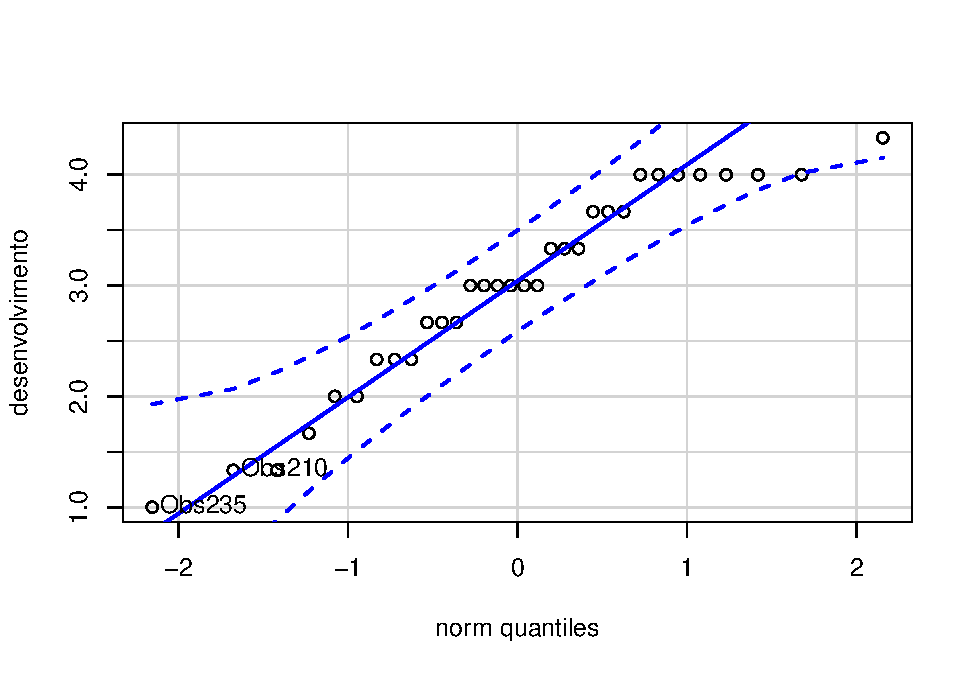
\includegraphics{factorialAnova_files/figure-latex/unnamed-chunk-29-1.pdf}

\begin{verbatim}
## Obs235 Obs210 
##     24     13
\end{verbatim}

\hypertarget{homogeneity-of-variance-assumption}{%
\subsubsection{Homogeneity of variance
assumption}\label{homogeneity-of-variance-assumption}}

\begin{Shaded}
\begin{Highlighting}[]
\KeywordTok{levene_test}\NormalTok{(sdat, }\StringTok{`}\DataTypeTok{desenvolvimento}\StringTok{`} \OperatorTok{~}\StringTok{ `}\DataTypeTok{area.de.conhecimento}\StringTok{`}\NormalTok{)}
\end{Highlighting}
\end{Shaded}

\begin{longtable}[]{@{}rrrll@{}}
\toprule
df1 & df2 & statistic & p & p.signif\tabularnewline
\midrule
\endhead
7 & 315 & 0.6285 & 0.7323 & ns\tabularnewline
\bottomrule
\end{longtable}

From the output above, non-significant difference indicates homogeneity
of variance in the different groups (Signif. codes: 0 **** 0.0001 ***
0.001 ** 0.01 * 0.05 ns 1).

\hypertarget{computation-anova}{%
\subsection{Computation ANOVA}\label{computation-anova}}

\begin{Shaded}
\begin{Highlighting}[]
\NormalTok{res.aov <-}\StringTok{ }\KeywordTok{anova_test}\NormalTok{(sdat, }\StringTok{`}\DataTypeTok{desenvolvimento}\StringTok{`} \OperatorTok{~}\StringTok{ `}\DataTypeTok{area.de.conhecimento}\StringTok{`}\NormalTok{, }\DataTypeTok{type =} \DecValTok{2}\NormalTok{, }\DataTypeTok{effect.size =} \StringTok{'ges'}\NormalTok{, }\DataTypeTok{detailed =}\NormalTok{ T)}
\KeywordTok{get_anova_table}\NormalTok{(res.aov)}
\end{Highlighting}
\end{Shaded}

\begin{verbatim}
## Coefficient covariances computed by hccm()
\end{verbatim}

\begin{longtable}[]{@{}lrrrrrllr@{}}
\toprule
Effect & SSn & SSd & DFn & DFd & F & p & p\textless{}.05 &
ges\tabularnewline
\midrule
\endhead
area.de.conhecimento & 7.863 & 218.676 & 7 & 315 & 1.618 & 0.13 & &
0.035\tabularnewline
\bottomrule
\end{longtable}

\hypertarget{post-hoct-tests-pairwise-comparisons}{%
\subsection{Post-hoct Tests (Pairwise
Comparisons)}\label{post-hoct-tests-pairwise-comparisons}}

\begin{itemize}
\tightlist
\item
  Estimated marginal means for \textbf{area.de.conhecimento}
\end{itemize}

\begin{Shaded}
\begin{Highlighting}[]
\NormalTok{(emm[[}\StringTok{"area.de.conhecimento"}\NormalTok{]] <-}\StringTok{ }\KeywordTok{emmeans_test}\NormalTok{(sdat, }\StringTok{`}\DataTypeTok{desenvolvimento}\StringTok{`} \OperatorTok{~}\StringTok{ `}\DataTypeTok{area.de.conhecimento}\StringTok{`}\NormalTok{, }\DataTypeTok{p.adjust.method =} \StringTok{"bonferroni"}\NormalTok{, }\DataTypeTok{detailed =}\NormalTok{ T))}
\end{Highlighting}
\end{Shaded}

\begin{longtable}[]{@{}lllrrrrrrrll@{}}
\toprule
.y. & group1 & group2 & estimate & se & df & conf.low & conf.high &
statistic & p & p.adj & p.adj.signif\tabularnewline
\midrule
\endhead
desenvolvimento & Ciências Agrárias & Ciências Biológicas & 0.2413 &
0.2374 & 315 & -0.2257 & 0.7084 & 1.0167 & 0.3101 & 1 &
ns\tabularnewline
desenvolvimento & Ciências Agrárias & Ciências da Saúde & -0.2374 &
0.1888 & 315 & -0.6088 & 0.1341 & -1.2572 & 0.2096 & 1 &
ns\tabularnewline
desenvolvimento & Ciências Agrárias & Ciências Exatas e da Terra &
-0.0099 & 0.1981 & 315 & -0.3997 & 0.3799 & -0.0501 & 0.9601 & 1 &
ns\tabularnewline
desenvolvimento & Ciências Agrárias & Ciências Humanas & -0.0997 &
0.2005 & 315 & -0.4943 & 0.2949 & -0.4973 & 0.6193 & 1 &
ns\tabularnewline
desenvolvimento & Ciências Agrárias & Ciências Sociais Aplicadas &
-0.0946 & 0.1947 & 315 & -0.4776 & 0.2884 & -0.4858 & 0.6274 & 1 &
ns\tabularnewline
desenvolvimento & Ciências Agrárias & Engenharias & -0.1071 & 0.2172 &
315 & -0.5345 & 0.3203 & -0.4932 & 0.6222 & 1 & ns\tabularnewline
desenvolvimento & Ciências Agrárias & Linguística/Letras e Artes &
-0.4301 & 0.2156 & 315 & -0.8543 & -0.0058 & -1.9946 & 0.0469 & 1 &
ns\tabularnewline
desenvolvimento & Ciências Biológicas & Ciências da Saúde & -0.4787 &
0.2059 & 315 & -0.8838 & -0.0735 & -2.3247 & 0.0207 & 0.5803 &
ns\tabularnewline
desenvolvimento & Ciências Biológicas & Ciências Exatas e da Terra &
-0.2513 & 0.2145 & 315 & -0.6733 & 0.1708 & -1.1713 & 0.2424 & 1 &
ns\tabularnewline
desenvolvimento & Ciências Biológicas & Ciências Humanas & -0.3411 &
0.2168 & 315 & -0.7675 & 0.0854 & -1.5736 & 0.1166 & 1 &
ns\tabularnewline
desenvolvimento & Ciências Biológicas & Ciências Sociais Aplicadas &
-0.3359 & 0.2113 & 315 & -0.7517 & 0.0799 & -1.5896 & 0.1129 & 1 &
ns\tabularnewline
desenvolvimento & Ciências Biológicas & Engenharias & -0.3485 & 0.2323 &
315 & -0.8055 & 0.1085 & -1.5004 & 0.1345 & 1 & ns\tabularnewline
desenvolvimento & Ciências Biológicas & Linguística/Letras e Artes &
-0.6714 & 0.2308 & 315 & -1.1254 & -0.2174 & -2.9096 & 0.0039 & 0.1086 &
ns\tabularnewline
desenvolvimento & Ciências da Saúde & Ciências Exatas e da Terra &
0.2274 & 0.1591 & 315 & -0.0856 & 0.5404 & 1.4296 & 0.1538 & 1 &
ns\tabularnewline
desenvolvimento & Ciências da Saúde & Ciências Humanas & 0.1376 & 0.1621
& 315 & -0.1813 & 0.4565 & 0.8490 & 0.3965 & 1 & ns\tabularnewline
desenvolvimento & Ciências da Saúde & Ciências Sociais Aplicadas &
0.1428 & 0.1547 & 315 & -0.1617 & 0.4472 & 0.9227 & 0.3569 & 1 &
ns\tabularnewline
desenvolvimento & Ciências da Saúde & Engenharias & 0.1302 & 0.1823 &
315 & -0.2285 & 0.4889 & 0.7142 & 0.4756 & 1 & ns\tabularnewline
desenvolvimento & Ciências da Saúde & Linguística/Letras e Artes &
-0.1927 & 0.1804 & 315 & -0.5476 & 0.1622 & -1.0683 & 0.2862 & 1 &
ns\tabularnewline
desenvolvimento & Ciências Exatas e da Terra & Ciências Humanas &
-0.0898 & 0.1729 & 315 & -0.4300 & 0.2503 & -0.5195 & 0.6038 & 1 &
ns\tabularnewline
desenvolvimento & Ciências Exatas e da Terra & Ciências Sociais
Aplicadas & -0.0846 & 0.1660 & 315 & -0.4113 & 0.2420 & -0.5099 & 0.6105
& 1 & ns\tabularnewline
desenvolvimento & Ciências Exatas e da Terra & Engenharias & -0.0972 &
0.1920 & 315 & -0.4749 & 0.2805 & -0.5064 & 0.6129 & 1 &
ns\tabularnewline
desenvolvimento & Ciências Exatas e da Terra & Linguística/Letras e
Artes & -0.4201 & 0.1901 & 315 & -0.7943 & -0.0460 & -2.2095 & 0.0279 &
0.78 & ns\tabularnewline
desenvolvimento & Ciências Humanas & Ciências Sociais Aplicadas & 0.0052
& 0.1689 & 315 & -0.3271 & 0.3375 & 0.0306 & 0.9756 & 1 &
ns\tabularnewline
desenvolvimento & Ciências Humanas & Engenharias & -0.0074 & 0.1945 &
315 & -0.3900 & 0.3752 & -0.0381 & 0.9696 & 1 & ns\tabularnewline
desenvolvimento & Ciências Humanas & Linguística/Letras e Artes &
-0.3303 & 0.1927 & 315 & -0.7094 & 0.0488 & -1.7145 & 0.0874 & 1 &
ns\tabularnewline
desenvolvimento & Ciências Sociais Aplicadas & Engenharias & -0.0126 &
0.1884 & 315 & -0.3832 & 0.3581 & -0.0668 & 0.9468 & 1 &
ns\tabularnewline
desenvolvimento & Ciências Sociais Aplicadas & Linguística/Letras e
Artes & -0.3355 & 0.1865 & 315 & -0.7025 & 0.0315 & -1.7986 & 0.0730 & 1
& ns\tabularnewline
desenvolvimento & Engenharias & Linguística/Letras e Artes & -0.3229 &
0.2100 & 315 & -0.7360 & 0.0902 & -1.5379 & 0.1251 & 1 &
ns\tabularnewline
\bottomrule
\end{longtable}

\hypertarget{descriptive-statistic-and-anova-plots}{%
\subsection{Descriptive Statistic and ANOVA
Plots}\label{descriptive-statistic-and-anova-plots}}

\begin{Shaded}
\begin{Highlighting}[]
\KeywordTok{get_summary_stats}\NormalTok{(}\KeywordTok{group_by}\NormalTok{(sdat, }\StringTok{`}\DataTypeTok{area.de.conhecimento}\StringTok{`}\NormalTok{), }\DataTypeTok{type =}\StringTok{"common"}\NormalTok{)}
\end{Highlighting}
\end{Shaded}

\begin{longtable}[]{@{}llrrrrrrrrr@{}}
\toprule
area.de.conhecimento & variable & n & mean & median & min & max & sd &
se & ci & iqr\tabularnewline
\midrule
\endhead
Ciências Agrárias & desenvolvimento & 28 & 2.560 & 2.333 & 1.333 & 4.333
& 0.720 & 0.136 & 0.279 & 1.000\tabularnewline
Ciências Biológicas & desenvolvimento & 22 & 2.318 & 2.333 & 1.000 &
4.333 & 0.832 & 0.177 & 0.369 & 1.333\tabularnewline
Ciências da Saúde & desenvolvimento & 64 & 2.797 & 3.000 & 1.333 & 4.333
& 0.760 & 0.095 & 0.190 & 1.000\tabularnewline
Ciências Exatas e da Terra & desenvolvimento & 48 & 2.569 & 2.667 &
1.000 & 4.333 & 0.891 & 0.129 & 0.259 & 1.417\tabularnewline
Ciências Humanas & desenvolvimento & 45 & 2.659 & 2.667 & 1.000 & 4.333
& 0.812 & 0.121 & 0.244 & 1.333\tabularnewline
Ciências Sociais Aplicadas & desenvolvimento & 53 & 2.654 & 2.667 &
1.000 & 4.333 & 0.867 & 0.119 & 0.239 & 1.333\tabularnewline
Engenharias & desenvolvimento & 31 & 2.667 & 2.667 & 1.000 & 4.667 &
0.873 & 0.157 & 0.320 & 1.333\tabularnewline
Linguística/Letras e Artes & desenvolvimento & 32 & 2.990 & 3.000 &
1.000 & 4.333 & 0.906 & 0.160 & 0.327 & 1.417\tabularnewline
\bottomrule
\end{longtable}

\begin{Shaded}
\begin{Highlighting}[]
\KeywordTok{ggPlotAoV}\NormalTok{(sdat, }\StringTok{"area.de.conhecimento"}\NormalTok{, }\StringTok{"desenvolvimento"}\NormalTok{, }\DataTypeTok{aov=}\NormalTok{res.aov, }\DataTypeTok{pwc=}\NormalTok{emm[[}\StringTok{"area.de.conhecimento"}\NormalTok{]], }\DataTypeTok{addParam=}\KeywordTok{c}\NormalTok{(}\StringTok{"jitter"}\NormalTok{))}
\end{Highlighting}
\end{Shaded}

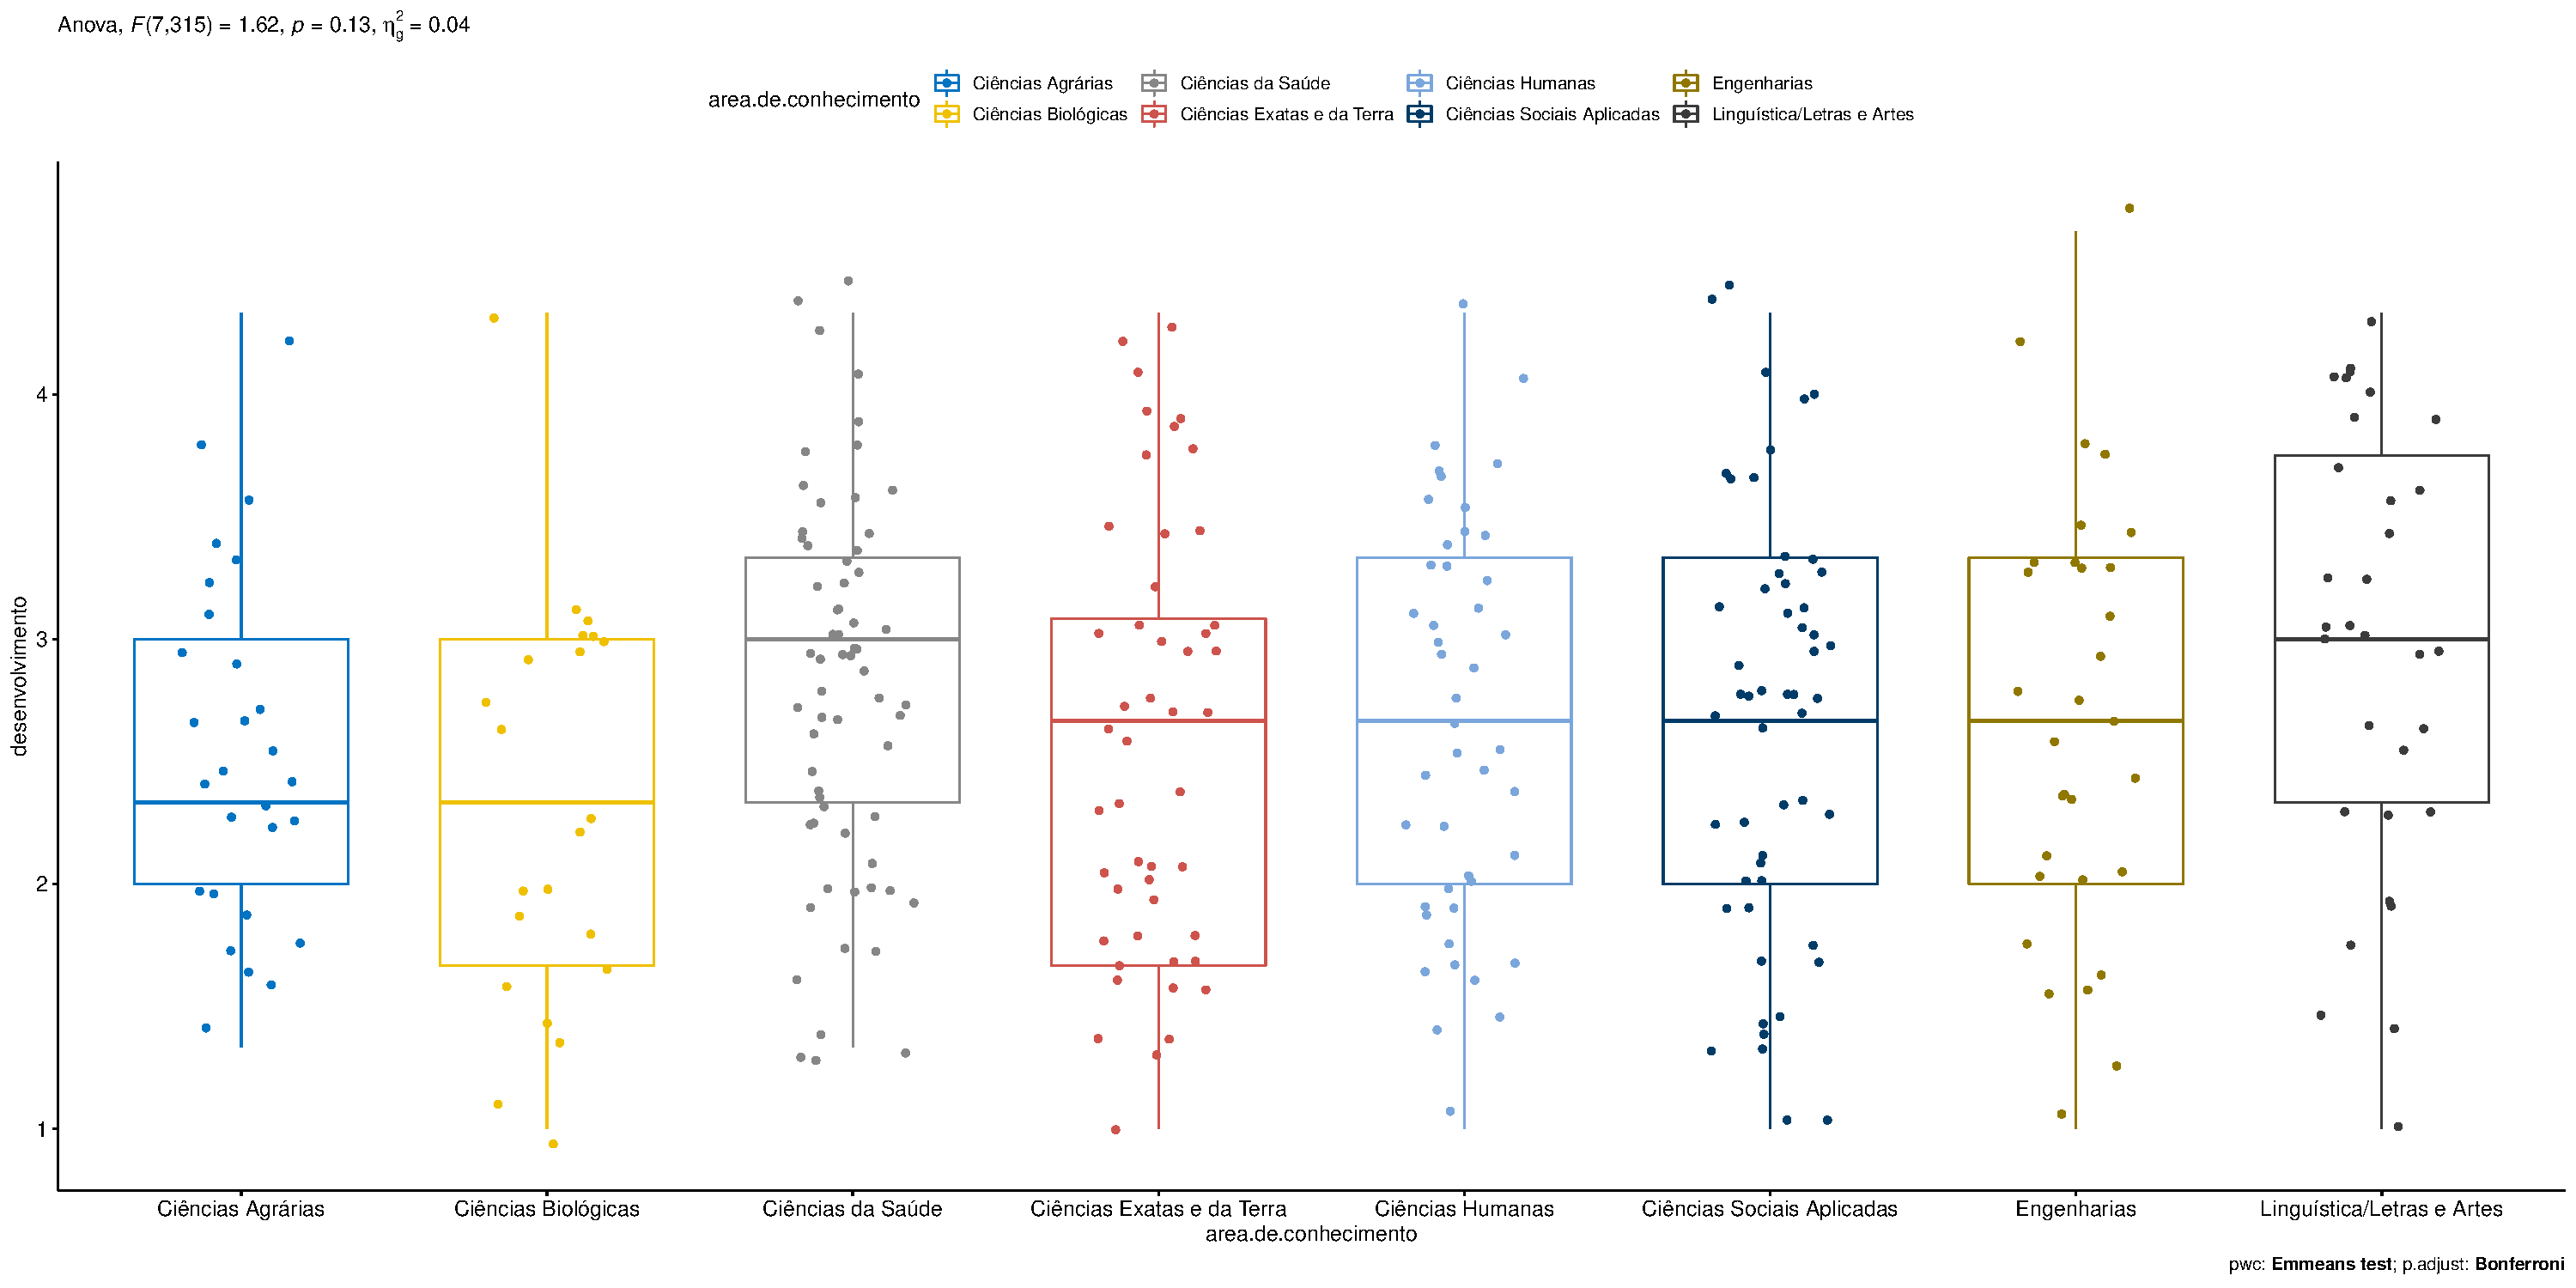
\includegraphics{factorialAnova_files/figure-latex/unnamed-chunk-34-1.pdf}

\hypertarget{references}{%
\subsection{References}\label{references}}

{[}1{]}: Blanca, M. J., Alarcón, R., Arnau, J., Bono, R., \& Bendayan,
R. (2017). Non-normal data: Is ANOVA still a valid option?. Psicothema,
29(4), 552-557.

{[}2{]}: Ghasemi, A., \& Zahediasl, S. (2012). Normality tests for
statistical analysis: a guide for non-statisticians. International
journal of endocrinology and metabolism, 10(2), 486.

{[}3{]}: Miot, H. A. (2017). Assessing normality of data in clinical and
experimental trials. J Vasc Bras, 16(2), 88-91.


\end{document}
